\documentclass[sans]{cdvreport}

\title{Definición y esquemas para el Simulador}
\author{Pablo Martín Yuste}
\doctype{Especificaciones Técnicas}

\begin{document}
\maketitle

\section{Aspectos generales del simulador}
El simulador consiste en el fuselaje de la cabina de un planeador \todo{Foto de un modelo del planeador del simu}, montada sobre una junta universal que permite los giros de cabeceo y alabeo, y dotado de dos motores eléctricos que mueven las articulaciones a la parte posterior del fuselaje.
\par El software empleado es \href{https://www.condorsoaring.com/}{Condor 3}, que permite una extracción de los datos del estado de vuelo del planeador mediante el protocolo UDP.
\par Este proyecto implementa un software para la extracción, interpretación y procesado de la telemetría de Condor 3, y lo combina con un hardware para controlar dinámicamente la actitud del planeador, con el objetivo de ofrecer una experiencia de vuelo realista.

\section{Sistemas del simulador}
El funcionamiento general del simulador se explica a continuación:
\begin{figure}[ht]
	\centering
	\begin{tikzpicture}
		%Nodos del diagrama de bloques
		\node[block] (condor3) {Condor 3};
		\node[block, below=1cm of condor3] (fisica) {Modelo de\\Física};
		\node[block, below=1cm of fisica] (kinematics) {Cinemática\\Inversa};
		\node[block, right=4cm of kinematics] (control) {Gestor\\USB};
		\node[block, above=1.8cm of control] (mcu) {MCU\\STM32F411};
		\node[block, left=1.3cm of mcu] (esc1) {Actuador 1};
		\node[block, right=1.3cm of mcu] (esc2) {Actuador 2};
		\node[block, above=0.5cm of mcu] (ess) {ESS};
		\node[above=0.5cm of ess] (vs) {24 V};
		\node[block, right=2cm of control] (logger) {Data logger\\Control manual};
		%Flechas del diagrama de bloques
		\path[line] (condor3.south) -- (fisica.north) node[midway, left] {\footnotesize Telemetría};
		\path[line] (fisica.south) -- (kinematics.north) node[midway, left] {$\theta, \phi$};
		\path[line] (kinematics.east) -- (control.west) node[midway, above] {$\psi_1, \psi_2$};
		\node[commbus, fill=cyan!20, shape border rotate=90, minimum height=1.8cm] at ($(control.north)!0.5!(mcu.south)$) {USB};
		\path[reline] (mcu.west) -- (esc1.east);
		\path[reline] (mcu.east) -- (esc2.west);
		\path[reline] (control.east) -- (logger.west);
		\path[line, draw=red] (vs.south) -- (ess.north);
		\path[line, draw=red] (ess.west) -| (esc1.north);
		\path[line, draw=red] (ess.east) -| (esc2.north);
	\end{tikzpicture}
\end{figure}

Como se puede observar, los datos brutos extraídos del Condor 3 pasan por dos tipos de procesado. En primer lugar la telemetría se convierte en unos ángulos de cabeceo y alabeo para el simulador real, utlizando un modelo de física que busca reproducir de la forma más fiel posible las fuerzas que se sentirían en cabina en las condiciones del vuelo simulado.
\par A continuación, un cálculo de cinemática inversa resuelve a qué posiciones se deben mover cada uno de los motores para alcanzar esa posición. Una vez determinadas estas posiciones, estos datos son pasados al gestor USB mediante un ciclo de control de alta frecuencia, para mover los motores.
\par El microcontrolador es responsable de implementar un algoritmo de control \todo{referencia cuando se explique este algoritmo} para mover los motores. Cada uno de los motores está instrumentado con un sensor de ángulo magnético para conocer exactamente su posición, permitiendo un control en bucle cerrado.
\par Como medida de protección activa, está presente un botón de desconexión de emergencia (ESS, \textit{Emergency Stop Switch}), que desactivará los puentes H e interrumpirá físicamente el suministro de corriente a los motores, permitiendo parar instantáneamente el movimiento del simulador. Además, el microcontrolador está conectado a este botón, indicando al software de escritorio esta detención.

\subsection{Aplicación de escritorio}
Para implementar de forma centralizada todo el código, se ha desarrollado una aplicación de escritorio responsable de preprocesar los datos de telemetría de Condor 3, y convertirlos en comandos de posición que enviar al sistema de control de los actuadores. Esta aplicación se ha desarrollado en Python, por sus facilidades para el desarrollo de la interfaz gráfica, con módulos individuales programados en \texttt{C++}. A continuación se explica detalladamente cada uno de sus componentes.

\subsubsection{Interfaz Gráfica}
Para facilitar el uso del software, se ha desarrollado una interfaz gráfica de uso general, que proporciona controles útiles, como activar o desactivar el sistema de movimiento, indicar si la telemetría se recibe correctamente de Condor 3, o controlar manualmente el simulador.

\subsubsection{Algoritmo de Generación de Movimiento}
\todo{Escribir detalladamente el funcionamiento del modelo de vuelo}
\par Se ha estudiado cómo implementar de la forma más satisfactoria el algoritmo de generación de movimiento para la plataforma del simulador. En primer lugar, se parte de alguno de los algoritmos de generación de movimiento genéricos \todo{referencia a una figura de MCA}. Después, se ha estudiado la forma más similar de adaptar la pose de una plataforma don 6 GDL a la del simulador, con solamente 2 GDL.
\par Actualmente, el principal problema consiste en resolver el ``Método de Tustin'', que permite traducir las ecuaciones del MCA, originalmente en el dominio de la frecuencia, a ecuaciones algebraicas en un esquema de diferencias finitas.

\subsubsection{Cinemática inversa}
\todo{Programar en \texttt{C++} para reducir el tiempo de ejecución y aumentar la fiabilidad del código.}
\par La cinemática inversa es el penúltimo proceso del cálculo de la posición de los actuadores. Consiste en, a partir de la actitud deseada para el planeador, resolver la posición y la velocidad de los actuadores.
\par Una explicación más detallada de este cálculo se puede encontrar en el \todo{referencia al anexo.}

\subsubsection{Gestor USB}
Esta parte de la aplicación de escritorio desarrollada se encarga de procesar los datos que deben transmitirse por la comunicación USB y recibir la información de estado que el microcontrolador devuelve. Se ha programado de forma independiente para poder gestionar eficientemente altos volúmenes de información.
\par \todo{Decidir si programar en Python o en \texttt{C++}}.

\subsubsection{Comunicación USB}
\todo{Definir comunicación}, qué datos van desde la app de escritorio, qué datos manda el microcontrolador de vuelta, cuál es la latencia objetivo de la comunicación, etc.

\subsection{Sistema de control del movimiento}
Externo a la aplicación de escritorio, y utilizando la conexión USB como comunicación, el sistema de control del movimiento consiste en toda la electrónica encargada de garantizar el movimiento de los actuadores de forma precisa y rápida. Los componentes se describen a continuación.
\par Se ha considerado como actuadores a todo el conjunto de puente H, motor y encoder magnético que está duplicado en el simulador. Cuando está conectado todo, el puente H recibe una señal PWM del microcontrolador que determina el par (y la velocidad) con la que el motor busca alcanzar la posición comandada. Para una representación general del funcionamiento de este subsistema, consultar la \autoref{fig:electronics-overview}

\begin{figure}[ht]
	\centering
	\begin{tikzpicture}
		\node[block, minimum width = 2.5cm] (mcu) {MCU\\STM32F411};
		\node[block, above=5mm of mcu] (ess) {ESS};
		\node[block, above=5mm of ess] (vplus) {24 \unit{\volt}};
		\node[polyarrow, fill=cyan!20, shape border rotate=90, minimum height=1.8cm, below=0mm of mcu] {USB};
		\node[block, left=1cm of mcu] (hb1) {BTS7960};
		\node[round, left=14mm of hb1] (Mo1) {Motor 1};
		\node[block, below=1mm of Mo1] (enc1) {MT6701};
		\node[block, left=7mm of hb1, anchor=south, yshift=3mm] (amp1) {Sens A};
		\node[block, right=1cm of mcu] (hb2) {BTS7960};
		\node[round, right=14mm of hb2] (Mo2) {Motor 2};
		\node[block, below=1mm of Mo2] (enc2) {MT6701};
		\node[block, right=7mm of hb2, anchor=south, yshift=3mm] (amp2) {Sens A};
		%Paths
		\draw[thick, red] (vplus.south) -- (ess.north);
		\draw[line, red] (ess.west) -| (hb1.north);
		\draw[line, red] (ess.east) -| (hb2.north);
		\draw[thick, red] ([yshift=1mm]hb1.west) -- ([yshift=1mm]Mo1.east);
		\draw[thick] ([yshift=-1mm]hb1.west) -- ([yshift=-1mm]Mo1.east);
		\draw[thick, red] ([yshift=1mm]hb2.east) -- ([yshift=1mm]Mo2.west);
		\draw[thick] ([yshift=-1mm]hb2.east) -- ([yshift=-1mm]Mo2.west);
		\draw[line] (mcu.west) -- (hb1.east) node[midway, above, textonly] {PWM};
		\draw[line] (mcu.east) -- (hb2.west) node[midway, above, textonly] {PWM};
		\draw[line] ([yshift=1mm]amp1.east) -| ([xshift=-5mm]mcu.north);
		\draw[line] ([yshift=1mm]amp2.west) -| ([xshift=5mm]mcu.north);
		\draw[line] (enc1.east) -| ([xshift=-10mm]mcu.south) node[midway, above left, textonly] {I2C};
		\draw[line] (enc2.west) -| ([xshift=10mm]mcu.south) node[midway, above right, textonly] {I2C};
		
	\end{tikzpicture}
	\caption{Funcionamiento general del sistema de control de movimiento}\label{fig:electronics-overview}
\end{figure}


\subsubsection{Microcontrolador}
\todo{Explicar qué código se ejecuta en el microcontrolador}, y qué algoritmos se emplean para el control de los motores (actuadores), si se implementa (o no) la regulación de la intensidad máxima...
\par Se ha elegido el \href{https://www.st.com/resource/en/datasheet/stm32f411ce.pdf}{STM32F411} por su alta frecuencia del microprocesador, además de tener disponibles dos buses I2C independientes, permitiendo una comunicación de milisegundos con los encoders magnéticos en paralelo.
\begin{figure}[ht]
	\centering
	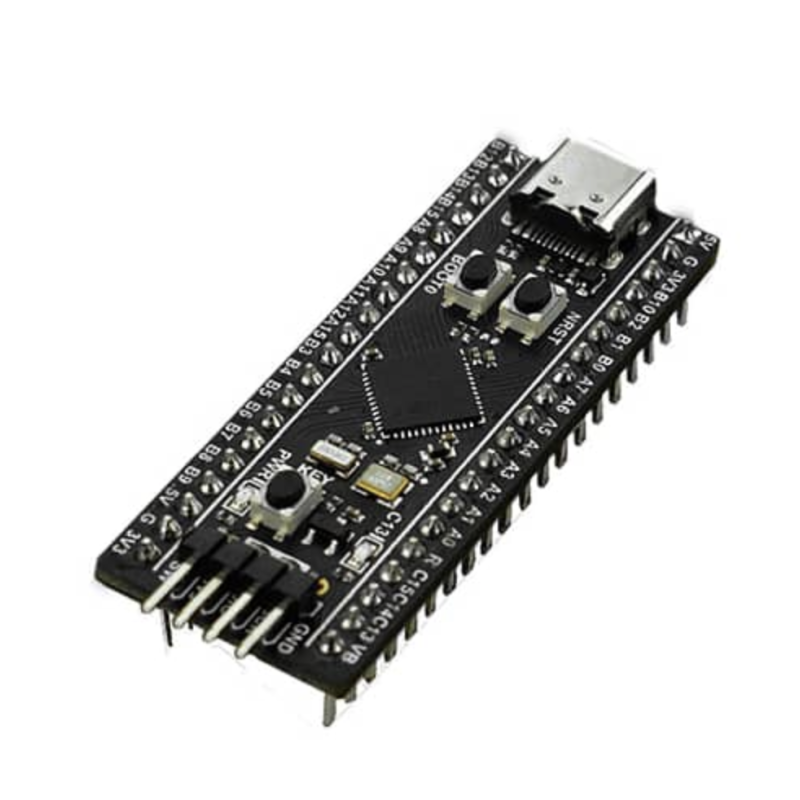
\includegraphics[width=0.4\textwidth]{figures/blackpill-mcu.jpg}
	\caption{Foto del microontrolador STM32F411}\label{fig:mcu-photo}
\end{figure}

\subsubsection{Puentes H BTS7960-43A}
Para poder conseguir un buen control de los motores, se utilizarán los puentes H BTS7960-43A para suministrar una tensión variable entre 0 y 24 \unit{\volt}. Estos componentes reciben una señal PWM (Pulse Width Modulation) del microcontrolador, y la utilizarán para polarizar de forma directa o inversa el motor, dando pulsos de tensión con el mismo \emph{duty cycle} que la señal PWM.
\\ \todo{Foto de los puentes h}.

\subsubsection{Motores}
Los motores son actuadores del parabrisas de un autobús, extraídos de un desguace. Se trata de motores de contínua de 24 V. Son capaces de proporcionar 16 Nm de par, con una reducción mediante tornillo sinfín.
\par \todo{Añadir foto de los motores}

\subsubsection{Encoders Magnéticos}
Para determinar con precisión la posición de cada uno de los motores, se están utilizando encoders magnéticos MT6701. Estos se comunican mediante el protocolo I2C al microcontrolador, con una precisión de 14 bits en la comunicación.
\\ \todo{Foto de MT6701 montado y sin montar}
\par \href{https://datasheet4u.com/pdf/1556274/MT6701.pdf}{Datasheet} del sensor.

\subsubsection{Fuentes de Alimentación}
Las fuentes utilizadas en este sistema son las DPS-600 PB. Estas son unas fuentes con un diseño propietario, por lo que no hay disponibilidad de manual de uso. Sin embargo, su uso es popular entre aficcionados al radiocontrol, y hay mucha información disponible en foros. 
\par \todo{Foto de las fuentes de alimentación}.
\\ \todo{Foto del pinout de las fuentes de alimientación}.

\section{Consideraciones}
\subsection{Control de Intensidad}
Experiencias pasadas con este sistema, utilizando algoritmos de control menos sofisticados, han demostrado que es frecuente que se exceda la intensidad máxima de trabajo de los actuadores, durante cambios bruscos de sentido (inversiones de carga). Esto puede provocar el colapso de los puentes H o daños en los devanados de los motores, por lo que es recomendable implementar instrumentación de medida de corriente, para añadir regulación en un futuro.

\subsection{Resensorización del simulador}
En el estado actual del simulador, las palancas físicas responsables del movimiento de los ejes de control está siendo gestionado por dos microcontroladores independientes: un LEO-BODNAR (antiguo) y un Arduino Pro Micro (más moderno). El LEO-BODNAR se encarga de los interruptores del tren de aterrizaje, mientras que el Arduino se encarga de los ejes de freno, guiñada y compensador.
\par Para evitar cableado y sistemas extra que no son necesarios, una posible mejora sería eliminar el controlador LEO-BODNAR y utilizar el Arduino Pro Micro para controlar todos los botones y ejes de la cabina. Además, los ejes cuya medida se hace ahora mediante potenciómetros, se deberían cambiar a sensores magnéticos de efecto de campo o encoders magnéticos, para aumentar la precisión y la vida de estos sensores.
\par La mejor propuesta para hacer esto consistiría en utilizar el multiplexor TCA9548A, conectado al Arduino para tener hasta 8 canales I2C con los que leer datos de encoders magnéticos, y considerar utilizar alguna de las matrices para botones que hay disponibles en el club.

\newpage
\listoftodos
\newpage

\appendix

\section{Resolución de la cinemática inversa}
\label{ax:inverse-kinematics}
\par La resolución de la cinemática inversa se hace en varios pasos. A continuación se explica el proceso para un actuador, pero evidentemente el cálculo se hace por duplicado al haber dos actuadores.
\begin{enumerate}
	\item Con los ángulos $\theta$ y $\phi$ obtenidos del modelo de vuelo, se calcula la matriz de rotación que permite convertir vectores de ejes cuerpo a ejes tierra. Para obtener esta matriz, se ha empleado el criterio mostrado en la \autoref{fig:rotacion-simu}

		\begin{figure}[!ht]
		\begin{center}
			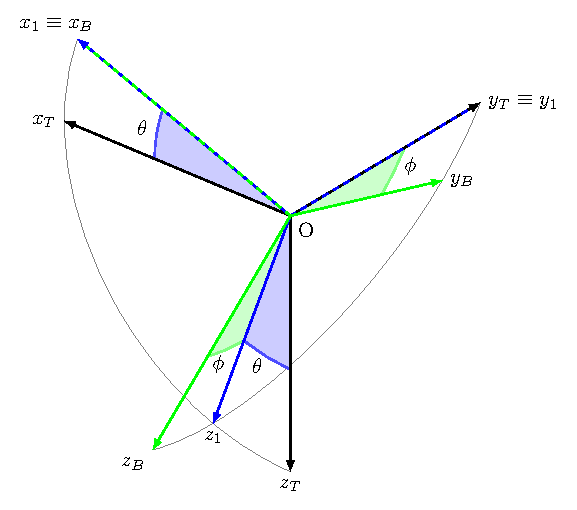
\includegraphics[width=0.5\textwidth]{figures/theta_phi.pdf}
		\end{center}
		\caption{Diagrama de la rotación mediante ángulos de Euler}\label{fig:rotacion-simu}
	\end{figure}

	\item Se calcula la posición final de los puntos $J$, los extremos de la barra horizontal unida al fuselaje a la que se unen las barras de las articulaciones. Con esto, se calcula la distancia del centro de cada motor (puntos $M$) a las juntas. Esta distancia será $l$.
	\item Con esto, los tres lados del triángulo formado por los lados $l$, $s$ y $t$ son conocidos, de forma que se puede emplear el teorema del coseno para calcular el ángulo ($\hat{S}$) que hay entre el lado $l$ y el lado $t$.
	\item A partir de las componentes $l_x$ y $l_z$ del vector $\vec{l}$, se puede calcular la longitud que tendrá el lado $l'$, que será la proyección del lado $l$ del triángulo en el plano $XZ$. De este triángulo, el lado $t$ también es conocido, porque este mismo lado está contenido siempre en el plano $XZ$.
	\item Aprovechando que la prependicularidad entre $b$, el segmento que es perpendicular a $l$ y pasa por el otro extremo de $t$, se conserva entre proyecciones\footnote{Esto no es una propiedad de la proyección, sino una particularidad por estar proyectando un triángulo que tiene un lado contenido en el plano $XZ$ a ese mismo plano.}, se puede resolver el triángulo $tp'b'$, ya que se conocen dos lados y un ángulo (ver \autoref{fig:triangle-projection})

	\begin{figure}[!ht]
		\begin{center}
		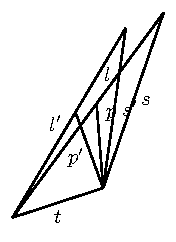
\includegraphics{figures/out/triangulos.pdf}
		\end{center}
		\caption{Representación de los triángulos $lst, btp$ y $b'p't$.}\label{fig:triangle-projection}
	\end{figure}
        \item Con el triángulo $b'p't$ resuelto, se puede calcular finalmente el ángulo que formará $t$ con la horizontal, resolviendo finalmente el ángulo $\psi$ del actuador.

\end{enumerate}

\end{document}
